\section{Die Daten}

Die zur Verfügung gestellten Daten bestehen aus 34.943 Bildern, wobei jeweils 25 Bilder einem Auge zugehörig sind. Auf einem Bild ist sowohl die Draufsicht des ganzen Auges, als auch jeweils einer der 25 Querschnitte zu sehen.

\begin{figure}[H]
\centering
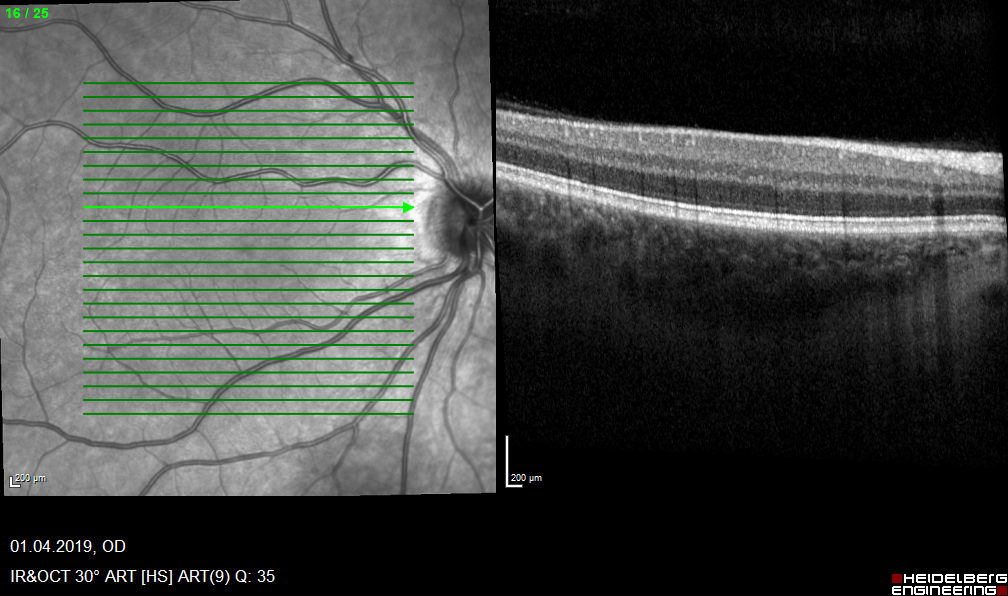
\includegraphics[width=0.7\textwidth]{./pic/Datenvorverarbeitung/OCT-Scan.png}
\caption{\label{fig:octscan}OCT Scan einer Schicht.}
\end{figure}

Die Draufsicht (Abb. \ref{fig:octscan} links) kann bei der Interpretation der Querschnitte hilfreich sein - der Großteil der relevanten Informationen für eine Ödemerkennung befindet sich jedoch auf den Querschnitten (Abb. \ref{fig:octscan} rechts).

In diesem Projekt werden die Querschnitte dennoch aus den Bildern extrahiert und die Draufsicht verworfen, um die Informationsdichte für das maschinelle Lernverfahren zu erhöhen. Dies wird automatisiert über die PIL Python library realisiert.

\section{Labeling}

Um den gewählten Supervised Learning Verfahren das Lernen aus den Daten zu ermöglichen, ist es notwendig, dass zuvor jedes Bild händisch klassifiziert und segmentiert wird. Für die Segmentierung dient das Tool VGG Image Annotator \cite{24}. Das Tool besteht aus einer browserbasierten Anwendung, mit der man die Bilder laden und Bereiche per Maus markieren kann (vgl. Abb. \ref{fig:vgg}) .

\begin{figure}[H]
\centering
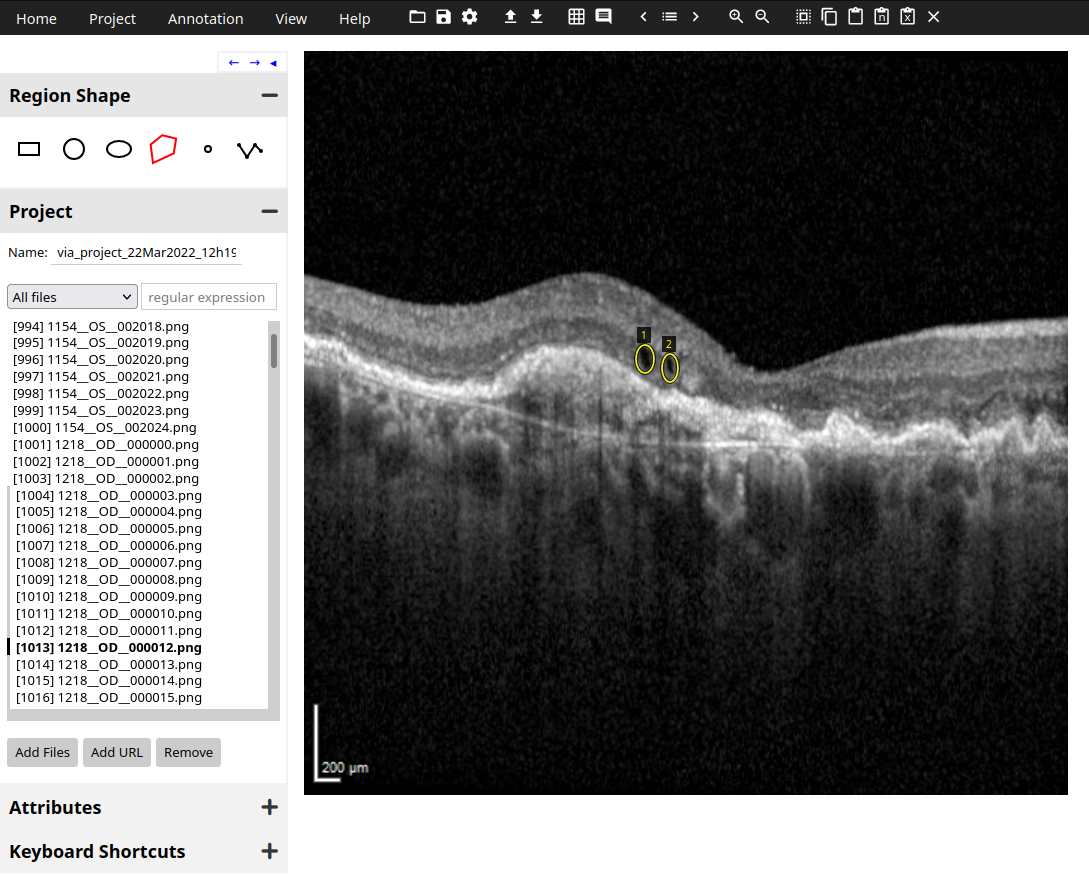
\includegraphics[width=0.7\textwidth]{./pic/Datenvorverarbeitung/VGG.png}
\caption{\label{fig:vgg}Labeln und Segmentieren eines Bildes im VGG Image Annotator}
\end{figure}

Um die Klassifizierung aus der Segmentierung zu gewinnen werden Klassenlabel für alle Bilder mit segmentierten Bereichen auf True und alle Bilder ohne segmentierte Bereiche auf False gesetzt. Dies ergibt 2.624 Bilder mit Ödem und 32.319 Bilder ohne Ödem. Dieses unausgewogene Verhältnis der Klassen und die geringe Menge an positiven Bildern bringt einige Probleme mit sich, wie einen Mangel an Trainingsdaten für die Segmentierung, welche nur auf positiven Bildern arbeitet, oder eine erschwerte Evaluierung.

Weitere Gegebenheiten die beim Labeling Verfahren die Qualität verringern sind ein Labeling basierend auf Laienwissen, unterschiedliche Labeler ohne stringende Labeling Richtlinien und ein Zeitmangel für die große Anzahl an Bildern.

\section{Datensätze}

\subsection{Datensätze für die Klassifikation}
Die gelabelten Bilder müssen nun noch in zwei getrennte Datensätze eingeteilt werden: Jene Daten die für das Training verwendet werden sowie Daten, welche für die anschließende Evaluierung der Performance auf ungesehenen Daten zurückgehalten werden. Aufgrund des unausgewogenen Verhältnisses der Bilder mit und ohne Ödem wird ebenfalls darauf geachtet, dass die Bilder stratifiziert auf die Datensätze aufgeteilt werden, also das Verhältnis an positiven und negativen Bildern auf beiden Datensätzen gleich gehalten wird. In Abb. \ref{fig:dataset_distribution} wird die Aufteilung der Trainings- und Testdaten für das Training und Testen des Klassifizierers vorgestellt.

\begin{figure}[H]
\centering
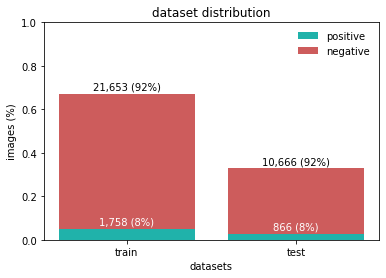
\includegraphics[width=0.6\textwidth]{./pic/Datenvorverarbeitung/classes.png}
\caption{\label{fig:dataset_distribution}Verteilung der Trainings- und Testdaten für die Klassifikation. Links ist der Trainingsdatensatz, rechts der Testdatensatz zu sehen. Die Anteile der Bilder mit Ödem (positiv) sind türkis dargestellt, die Anteile der Bilder ohne Ödem (negativ) sind rot eingefärbt.}
\end{figure}

\subsection{Datensätze für die Segmentierung}
Das Training der Segmentierung wird ausschließlich auf Bildern mit Makulaödemen (positiv) vorgenommen. Daher wurden separate Trainings-und Testdatensätze für die Segmentierung erstellt.\newline
Da im Training ausschließlich positive Bilder verwendet werden können und der Datenumfang entscheidend für den Trainingserfolg sein kann, wurde ein Trainings-/Testsplit gewählt, bei dem ein Großteil der Bilder im Trainingsdatensatz verwendet werden.
% Test: insg. 50 pos, alle negative
% Trainig: alle positiven Bilder minus 50


Um das Mask R-CNN trainieren zu können, werden als Input-Daten neben den Bildern auch die Masken der Ödeme im Bild benötigt. Dafür wird für alle mit dem VGG Image Annotator von Hand segmentierten OCT-Bilder, die Fläche der Ödeme berechnet und anschließend über die Pixelmenge innerhalb der Fläche die Maske erstellt. 
Die Masken, die im Training übergeben werden, enthalten nun nur noch die Pixelfläche der segmentierten Ödeme eines OCT-Scans. Je nachdem wie viele Flüssigkeitsansammlungen auf einem OCT-Scan von Hand segmentiert wurden, kann eine Maske ein oder mehrere Flächen enthalten. 
In Abbildung \ref{input_mrcnn} sind beispielhafte Input-Daten abgebildet. 

\begin{figure}[H]
\centering
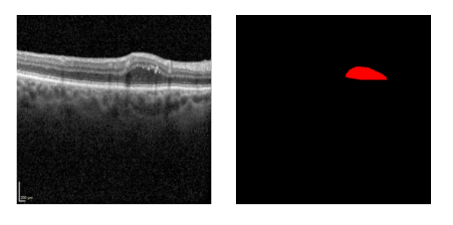
\includegraphics[width=100mm,scale=1.5]{pic/Segmentierung/input_mrcnn.png}
\caption{\label{input_mrcnn}Input-Daten des Mask R-CNN (Links: OCT-Bild, Rechts: Maske des Ödems)}
\end{figure}

Für das Training wurden die Daten in Trainings- und Validierungsdatensatz in einem Verhältnis von 80:20 aufgeteilt. Die beiden Input-Datensätze bestehen wiederum aus den OCT-Bildern sowie deren Masken (vgl. Abb.\ref{aufteilung_data}). 

Da für das Trainieren nur die OCT-Bilder auf denen sich ein Ödem befindet verwendet werden können, werden insgesamt 5598 Bilder aus dem gesamten Datensatz von 34.948 OCT-Bildern berücksichtigt. 
Von dem Trainingsdatensatz werden 50 Bilder entnommen, die später für das Testen des Modells verwendet werden. 
Somit befinden sich 4439 Bilder im Trainingsdatensatz und 1109 im Validierungsdatensatz. 

Das Mask R-CNN wurde mit den beschriebenen Datensätzen für 10 Epochen auf Cloud-Ressourcen von Amazon-Web-Services trainiert. Im folgenden Abschnitt wird die Verwendung von AWS näher beschrieben. 


\begin{figure}[H]
\centering
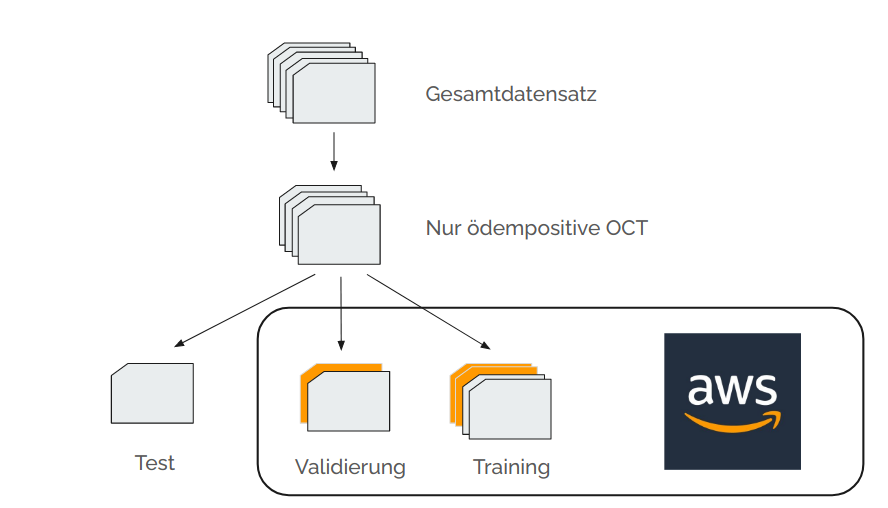
\includegraphics[width=0.7\textwidth]{pic/Segmentierung/training_segmentation.png}
\caption{\label{aufteilung_data}Aufteilung der OCT-Bilder für das Training des Mask R-CNN}
\end{figure}

\section{Training auf AWS}

Da aufgrund der hohen Datenmenge eine hohe Rechenkapazität notwendig ist, wird das Training der CNN jeweils für die Klassifikation und die Segmentierung auf Cloud-Ressourcen von Amazon Web Services durchgeführt. 
Das Training würde auf privaten Rechnern aufgrund der zu geringen Rechenkapazität schlicht von zu langer Dauer sein.
Die genutzte p2.xlarge Instanz von AWS verfügt über eine K80-GPUs von NVIDIA, 4 CPUs und 61 GB RAM, und ist somit speziell für die Berechnung von Deep Learning Verfahren ausgelegt.  (vgl. \cite{15}) 
Als persistentes Speichermedium, auf dem die Daten für das Training sowie dessen Ergebnisse abgelegt werden, wird ein S3 Bucket von AWS verwendet.